\documentclass[10pt,conference]{IEEEtran}
\usepackage[utf8]{inputenc}
\usepackage[T1]{fontenc}
\usepackage{hyperref}
\hypersetup{colorlinks=true,urlcolor=black,linkcolor=black,citecolor=black}
% \usepackage{subfig}
\renewcommand{\sectionautorefname}{Section}
\usepackage{enumitem}
\usepackage{balance}
\usepackage{xcolor}
\usepackage{graphicx}
\usepackage{booktabs}
% \usepackage{adjustbox}
\usepackage{multirow}
\usepackage{comment}
\usepackage{threeparttable}
\usepackage{microtype}
\usepackage{relsize,xspace}
\usepackage{cite}
\usepackage{textcomp}
\usepackage{mdframed}
\usepackage{framed}
\usepackage{enumitem}
\usepackage{MnSymbol,wasysym}
\usepackage{subfigure}
\usepackage{mdframed}
\usepackage{framed}
\usepackage{float}
\usepackage[normalem]{ulem} % [normalem] prevents the package from changing the default behavior of `\emph` to underline.


% \usepackage[dvipsnames]{xcolor}


\usepackage{listings}
\usepackage{caption}

%\usepackage{minted}
\usepackage{color, soul}

\definecolor{dark_green)}{rgb}{0.0, 0.5, 0.0}

\newcommand{\tm}[1]{{\color{blue}\textsf{TM}[\smaller\sffamily #1}]}
\newcommand{\az}[1]{{\color{orange}\textsf{AZ}[\smaller\sffamily #1}]}
\newcommand{\jb}[1]{{\color{red}\textsf{JB}[\smaller\sffamily #1}]}
\newcommand{\sd}[1]{{\color{magenta}\textsf{SD}[\smaller\sffamily\color{magenta} #1}]}
\newcommand{\ad}[1]{{\color{violet}\textsf{AD}[\smaller\sffamily #1}]}
\newcommand{\cd}[1]{{\color{cyan}\textsf{CR}[\smaller\sffamily #1}]}

\newcommand{\java}{\textsf{Java}\xspace}
\newcommand{\cp}{\textsf{C}\xspace}
\newcommand{\cpp}{\textsf{C++}\xspace}
%\newcommand{\java}{\textsf{Java}\xspace}
\newcommand{\py}{\textsf{Python}\xspace}
\newcommand{\rb}{\textsf{Ruby}\xspace}
\newcommand{\go}{\textsf{Go}\xspace}
\newcommand{\librariesio}{\textsf{Libraries.io}\xspace}

\newcommand{\git}{\textit{git}\xspace}
\newcommand{\rqOne}{$RQ_1$ Do the variant forks and their upstream counterparts have common maintainers?}
\newcommand{\rqOneOne}{$RQ_{1.1}$ \emph{How many of the original developers of the mainline maintained the variant in its first 6 months?}}
\newcommand{\rqOneTwo}{$RQ_{1.2}$ \emph{Do the variant and mainline have common active maintainers?}}
\newcommand{\rqTwo}{$RQ_{2}$ What was the motivation for creating the variant fork of an upstream project?}
\newcommand{\rqTwoOne}{$RQ_{2.1}$ \emph{Was the motivation for creating the variant an individual or a community decision?}}
\newcommand{\rqTwoTwo}{$RQ_{2.2}$ \emph{What was the motivation for creating the variant of the mainline project?}}
\newcommand{\rqTwoThree}{$RQ_{2.3}$ \emph{What are the motivation details relating to the motivation in $RQ_{2.2}$?}}
\newcommand{\rqThree}{$RQ_{3}$ Do the upstream and variant fork still interact?}
\newcommand{\rqThreeOne}{$RQ_{3.1}$ \emph{Do the variant forks and the upstream still discuss the main directions of the project?}}
\newcommand{\rqThreeTwo}{$RQ_{3.2}$ \emph{Do the variant developers integrate changes to and from the upstream repository?}}

\newcommand{\gh}{GitHub\xspace}
\newcommand{\ra}{\ensuremath{\rightarrow}}
\newcommand{\nd}{\vspace{1mm}\noindent}

\makeatletter
\def\endthebibliography{%
  \def\@noitemerr{\@latex@warning{Empty `thebibliography' environment}}%
  \endlist
}
\makeatother



\begin{document}

\title{Motivations Behind Variant Forks Creation and Maintenance}

% \author{\IEEEauthorblockN{John Businge,\IEEEauthorrefmark{1}
% 		Alexandre Decan,\IEEEauthorrefmark{2}
% 	Ahmed Zerouali,\IEEEauthorrefmark{3}
% 	Tom Mens\IEEEauthorrefmark{2} and
% 	Serge Demeyer,\IEEEauthorrefmark{1}}
% 	\IEEEauthorblockA{\IEEEauthorrefmark{1}University of Antwerp, Antwerp, Belgium}
% 	\IEEEauthorblockA{\IEEEauthorrefmark{2}University of Mons, Mons, Belgium}
% 	\IEEEauthorblockA{\IEEEauthorrefmark{3} Vrije Universiteit Brussels, Brussels, Belgium}
% 	}

\maketitle

\begin{abstract}
Some developers are reusing existing software software (OSS) hosted on social coding platforms by splitting-off a new development branch, often to steer the development into another direction, without the intention to  contribute back. We call these kind of forks variants of the original (mainline) projects.
We conduct an exploratory study on variant forks to understand the motivations behind variant fork creation and maintenance. Our study is based on a survey conducted on 112 maintainers of 105 active OSS variants projects hosted on GitHub a very popular social coding platform. Our study confirms and extends the findings of previous studies. Among the findings, we identify a number of fine-grained motivations behind the creation and maintenance of variants. We also identify concrete reasons why there is limited interaction between the mainline and variant projects. Based on our findings, we discuss future research direction in the line of efficient software reuse between the variants and the mainline counterparts.
\end{abstract}

\begin{IEEEkeywords}
Mainlines, Variants, GitHub, Software ecosystems, Maintenance, Variability
\end{IEEEkeywords}

\section{Introduction}
\label{sec:intro}
There is an increasing popularity of maintaining open source projects on social coding platforms like \gh. This has substantially improved both code reuse and collaborative development through forking of software repositories as well as sharing of code changes though pull requests and many \git facilities available.
A developer may fork a \textit{mainline repository} into a new \textit{forked repository}, typically transforming governance over the latter to a new developer, while preserving the full revision history and establishing traceability information. 
Forking was rare and was typically intended to compete with the original project~\cite{Linus:2012Perspectives,Gregorio:2012,Viseur:2012Forks,Linus:2013CodeForking,Linus:2011ToFork,Gamalielsson:2014Sustainability}.
The community typically distinguishes between two kinds of forks~\cite{Zhou:2020}.
\textit{Social forks} that are created for isolated development with the goal of contributing back to the mainline. \textit{Variant forks} that are created for splitting off a new development branch, often to steer the development into another direction without intending to contribute back, while leveraging the mainline project that defines or adheres to some standards~\cite{sung:ICSE:2020}.

A lot of studies have already investigated variant forking of free and open-source projects focusing on identifying the motivations behind variant forks~\cite{Linus:2012Perspectives,Gregorio:2012,Viseur:2012Forks,Linus:2013CodeForking,Linus:2011ToFork,Gamalielsson:2014Sustainability}. However, most of these studies has been conducted before the rise of social coding, much of it on \texttt{SourceForge}, before the popularity of social coding platforms like \gh. 
We know of only two studies that have so far investigated reasons for forking~\cite{businge:2018icsme,Zhou:2020}. Zhou et al.~\cite{Zhou:2020} report that perceptions and practices of variant forking in the \gh era changed significantly. Variant forks often evolve out of social forks rather than being planned deliberately and developers frequently perceive them as alternatives to the original projects.

This study builds on the previous studies to further investigate the motivations behind the creation and maintenance of variants on \gh the largest social coding platform. To achieve our goal, we performed an exploratory investigation of maintainers of variants hosted on \gh. We conducted an online survey that was answered by 112 maintainers of active variant projects.

\nd \textbf{We report a number of findings}: 1) Our study confirms the findings of a previous study that carried out an a large scale quantitative investigation on variants on \gh, that reported that most variants are maintained by developers not common to those in mainline counterparts. 
2) Our study also confirms other previous studies on motivations for creating variants. However, our study also extends the findings of these previous studies by providing more fine-grained motivations for creating variants. Furthermore, our study has also identified other motivations for creating and maintaining variants not listed in literature. 
3) Our study has also identified a number of categories relating to different reuse practices of variants. For example, we have discovered software reuse of a family of applications from the ``cryptocurrency world'', which is dedicated project software ecosystem. 
4) Our study confirms the findings of a previous study that carried out an a large scale quantitative investigation on variants on \gh, that reported that there is little code propagation between mainline and variants. Furthermore, our study extends the previous study by providing concrete reasons relating to the little code integration observed. For example, technically diverged variants, such as, those targeting different goals, those implementing different technologies, and those maintaining a specific feature of a mainline that was abandoned (a frozen feature). Based on these categories of variants, we have also discussed implications to tool building can help aid efficient code reuse between the mainlines and diverged variants.


\section{Background and Related Work}
\label{sec:background}
We discuss related work on: (i) motivations for creating\,/\,maintaining a variant fork and (ii) interaction between variant fork and mainline%, and (iii) general studies on variant forking.

\subsection{Motivations for creating\,/\,maintaining a variant fork}
\label{sec:motivations}
There are existing studies that have investigated motivations for creating\,/\,maintaining variant forks. However, most of these studies were carried out in the pre-\gh days of \texttt{SourceForge}, before the advent of social coding environment~\cite{Linus:2012Perspectives,Gregorio:2012,Viseur:2012Forks,Linus:2013CodeForking,Laurent:2008,Linus:2011ToFork}. While studies reports controversial perceptions around variant forks in the pre-\gh days~\cite{Chua:Forking:2017,Dixion:2009Forks,Ernst:2010,Linus:2011ToFork,Linus:2014Hackers,Raymond:Cathedral:2001}, Zhou et al.~\cite{Zhou:2020} reports that these perceptions have changed with the advent of \gh. Jiang et al.~\cite{Lo:2017} state that, although forking is controversial in traditional open source software (OSS) community, it is encouraged and is a built-in feature in \gh. Jiang et al. ~\cite{Lo:2017} further report that developers fork repositories to submit pull requests, fix bugs, add new features and keep copies (these of forks are called social forks). Zhou et al.~\cite{Zhou:2020} also report that most variant forks start as social forks. 
Robles and Gonz{\'a}lez-Barahona~\cite{Gregorio:2012} carried out a comprehensive study on a carefully filtered list of 220 potential forks that were referenced on Wikipedia. The authors assumed that a fork is significant if a reference to it appears in the English Wikipedia.
There are quite a number of identified reasons for creating variant in literature, however in this study we are only interested in those where both the mainline and variant co-evolve together. Below we present the reported reasons. 

\begin{list}{$\circ$}{}
   \item \textit{Technical reasons.} refer to adding or focusing content---for instance, when a developer wants to include a new feature in the mainline, but the mainline developers are reluctant to do so. An example is \texttt{Poppler} a fork of \texttt{xpdf}~\cite{Gregorio:2012}. \texttt{Poppler} is a customized version of \texttt{xpdf} with the use of the poppler library~\cite{poppler}.
    
    
    \item \textit{Governance disputes.} This may occur when the original leaders (e.g., a company, an institution or an independent group of developers) do not take into account the community. An example is \texttt{GNU XEmacs} as a fork of \texttt{GNU Emacs}.
    The fork \texttt{GNU XEmacs} (originally Lucid), was created as a result of the significant delays occurred in bringing out a new version of \texttt{GNU Emacs}~\cite{XEmacs}. Lucid Inc. was faced a requirement to ship \texttt{GNU Emacs} to support the Energize \texttt{C++} IDE. So Lucid recruited a team to improve and extend \texttt{GNU Emacs} and to-date \texttt{GNU XEmacs} is still being maintained. Another example The developer team disagrees on fundamental issues (beyond mere technical matters) related to the software development and the project, causing the team to split into different projects. The \texttt{OpenBSD} fork from \texttt{NetBSD} is an example of such a type of fork~\cite{openbsd}.


   % \item \textit{Reviving an abandoned project}. When the original project is not maintained and a new developer community wishes to take over its maintenance. For example, \texttt{NCSA httpd} project to \texttt{Apache Web server} project. NCSA abandoned its web server \texttt{httpd}, then some of its users banded together to maintain it. This resulted into the world’s most popular web server, \texttt{Apache Web server}~\cite{Wheeler:2015Forking}.

   % \item \textit{Commercial strategy}. When a company forks an existing project to meet some commercial strategy. 

\item \textit{Legal issues}. A project might consider different licenses, a trademark dispute may arise, or changes in laws (e.g., regarding encryption) require technical changes. Variant forks can be used to split development for different jurisdictions. Legal issues may also relate to commercial strategy. Commercial strategy forks include those where a software is released as free software by the company, or when the company creates a proprietary version of a free software. An example of such a fork is \texttt{OpenOffice} from \texttt{StarOffice}. In 1999, Star Division owned \texttt{StarOffice}, then the latter was acquired by Sun Microsystem for 59.5 million US dollars as it was supposedly cheaper than licensing Microsoft Office for 42,000 staff members. \texttt{OpenOffice} was forked from as \texttt{StarOffice} in 2000. After the fork, subsequent versions of \texttt{StarOffice} were based on additional proprietary components~\cite{Openoffice}.

\item \textit{Personal}: Interpersonal disputes and irreconcilable differences of a non-technical nature lead to a rift between various parties, hence the project forks. OpenBSD is a classic example~\cite{Zhou:2020}.

%The variant was created because some of the contributors felt that their feedback was not heard or maintainers were accepting patches too slowly in the mainline project.

% \item \textit{Experimental}: Creating a fork to try out and test new features that will be integrated into the mainline. This category can be seen as a subcategory of technical reasons.
\end{list}

The work in this study compliments the studies of Businge et al.~\cite{businge2018appfamilies} and  Zhou et al.~\cite{Zhou:2020} who have so far investigated variant forking in \gh. Businge et al.~\cite{businge2018appfamilies} studied forking motivations for only 11 variant forks from the Android ecosystem. The authors reported motivations for creating a variant fork of an Android app that includes: re-branding and simple customizations, feature extension and implementation of different but related features.  
Zhou et al.~\cite{Zhou:2020} interviewed 18 developers of hard forks on \gh to understand reasons for forking in more modern social coding environments that explicitly support forking. The authors reported that the motivations they observed align with the findings of prior (mentioned above ) studies. 

Another recent study that has investigated variant forks is that of Sung et al.~\cite{sung:ICSE:2020}. The authors conducted an industrial case study of the implications of frequent merges from mainline and the resulting merge conflicts in a variant fork. They implemented a tool that can automatically resolve up-to 40\% of the list of eight mainline induced build breaks. 

While the pre-\gh studies reported controversial perceptions around variant forks, Zhou et al.~\cite{Zhou:2020} report that these perceptions have changed with the advent of \gh. Jiang et al.~\cite{Lo:2017} state that, although forking is controversial in traditional open source software (OSS) communities, it is actually encouraged as a built-in feature in \gh. The authors further report that developers fork repositories to submit pull requests, fix bugs, add new features and keep copies (social forks).
Zhou et al.~\cite{Zhou:2020} also report that many variant forks actually start as social forks. 

\subsection{Interaction between variant fork and mainline}
We have only come across the study of Zhou et al.~\cite{Zhou:2020} that has investigated interaction between variant fork and mainline.
%\az{I think we need to define the mainline here first. Maybe also define the used terms in a subsection "terminology". For example mainline} \jb{The only terminologies we have are variants and mainline. I plan to define them in the introduction section}
In a study the authors conducted 18 semi-structured interviews with developers. They reported that many interviewees indicate that they are interested in coordinating across repositories, either for merging some or all changes back mainline eventually or to monitor activity in the mainline repository to incorporate select or all changes. Another study that has investigated interaction between mainline and variant is that of Businge et al.~\cite{businge:emse:2021}. The authors quantitatively investigated code propagation among variants and mainline from three software ecosystems. They found that only about 11\% of the 10,979 mainline--variant pairs had integrated code between themselves. Like Zhou et al.~\cite{Zhou:2020}, in this study we carry out a qualitative study to find out if variant developers integrate code to and from the mainline repositories.

%\subsection{General studies on variant forking}
% Like the between variant fork and mainline, we did not find many studies that relate to general studies on variant forking.
% One recent study that we came across investigated variant forks is that of Sung et al.~\cite{sung:ICSE:2020}. The authors conduct an industrial case study of the implications of frequent merges from mainline and the resulting merge conflicts in a variant fork. They implemented a tool that can automatically resolve up-to 40\% of the list of eight mainline induced build breaks. \az{the last two paper mentioned are already discussed above.}

\section{Research Questions}
\label{sec:rqs}

Our examination of the literature revealed that while several
studies have investigated variant forks, only a limited number has been performed on \gh.
No work has extensively examined the motivations behind creating variant forks in the \gh days.
To this end, the overall goal of this research is to understand the developers' motivation behind creating a variant fork in the context of social coding platforms like \gh. We also want to understand if the variant forks and their upstream repositories continue collaboration during the co-evolution. 
Consequently, our first question explores the developers' motivation behind creating a variant fork.

\nd  \textbf{\rqOne} With this research question, we aim to investigate if the creators of the variant were part core developers of upstream or not, and whether the upstream and variant currently have active maintainers.

\nd  \emph{\rqOneOne}

\nd \emph{\rqOneTwo}

\nd \textbf{\rqTwo} With this research question, we want to investigate if the motivations reported in literature (see Section~\ref{sec:background}) still hold or there are new ones in this \gh era.
To understand the motivations behind the creation and maintenance of variant forks, we ask two questions:

\nd \textit{\rqTwoOne} 

\nd  \textit{\rqTwoTwo} 

\nd  \textit{\rqTwoThree}

\nd \textbf{\rqThree} In Section~\ref{sec:background}, the literature based on quantitative analysis of variants from three ecosystems revealed that there is limited interaction between variants and upstream repositories. With this research question, we want to ascertain if this holds by performing a qualitative study. We asked the following subquestions.

\nd \textit{\rqThreeOne}

\nd \textit{\rqThreeTwo}

\section{Study Design}
\label{sec:study_design}
To understand the motivations behind the creation and maintenance of variant forks we performed the following activities: first, we collected mainline--variant fork pairs from \gh and then extracted the participants from the variant forks. Next, we designed and developed a survey protocol that we used to recruit the participants.
 %The survey was run in April 2021 with the goal of understanding why developers create and maintain variant forks.


 \ad{@John: I suggest to first explain how you designed the survey, then how you found/selected participants, then how you analyzed their answers.}


\subsection{Identifying variant Forks and Participants}
\label{sec:forks_and_participants}

\ad{I think there are too many (technical and practical) details in this section. This is likely to confuse the readers. I propose to focus on the main steps only, and to better motivate what we did. I propose the following outline: to conduct the survey, we need developers involved in the creation and maintenance of variant projects; to identify potentially competing variant projects; we distinguish between \emph{attached} and \emph{detached} projects; we relied on two data sources, namely Libraries.io and \gh; Libraries.io contains metadata for distributed packages on various package registries; we extracted the metadata and filtered those projects that are forks of another one using \gh API; we also used \gh search feature to find popular repositories and their forks; we manually filtered repositories corresponding to mainline projects and their variant projects; at the end of this step, we have XX \emph{attached} mainline-variant pairs; we also used \gh search feature looking for repositories that are not referred as ``forks'' but that do contain ``fork of'' in their description; at the end of this process, we have XX \emph{detached} mainline-variant pairs we manually checked; then we looked at the project history to find appropriate respondent candidates (how?); we contacted them, and got XX responses.}

Like we discussed in Section~\ref{sec:intro} we stated that a variant fork of an mainline project is also a real product developed in parallel with the mainline, while providing a solution different from the mainline.
We extract our dataset variant forks from two main sources: the first dataset is extracted from \librariesio\footnote{https://libraries.io} and and the second dataset is extracted directly from \gh. We further classify the second dataset into two types: ones where the variant fork is still attached to the mainline (a direct traceability link between mainline and fork still exists that can be used for exchanging pull requests), and variant forks which are detached from the mainline (no direct traceablity link exists).

\subsubsection{Libraries.io}
\label{sec:library.io}
We extracted the mainline--variant fork pairs from the most popular package managers for different programming language ecosystems that can be found on one central location \librariesio, which is a platform that periodically collects all data from different package managers, that include, \texttt{npm}, \texttt{Go}, \texttt{Maven}, \texttt{Plpy}, \texttt{Packagist}, etc. We extract the mainline--variant fork pairs from the latest \texttt{Libraries.io} data dump release 1.6.0 that was released on January 12, 2020. The meta-model for the data on the \texttt{Libraries.io} data dump can be found online.\footnote{https://libraries.io/data}
We follow the following steps:

\begin{enumerate}[label=\alph*.]
\item  Using the package's field \texttt{Platform}, we filter out the packages that are distributed on popular package managers.

\item Next, we use the field \texttt{Forkboolean} to identify repositories that are forks, and use the field \texttt{Fork Source Name with Owner} to identify the fork repository name as well as the parent repository (mainline).

\item Next, we merge the sets of packages from Step 1 and Step 2 to identify only packages that make an mainline--fork pair (i.e., where the fork repository and its corresponding mainline in the set in Step 2 have their packages present in the set in Step 1. Using the \gh API, we then verify that indeed the mainline is a parent of the variant fork and they are still existing on \gh so as to eliminate wrong pairs (e.g., those that have been deleted from \gh).

\item Using the \gh API, we then verify that indeed the mainline parent and the fork variant are still existing on \gh. We also extract the latest commit dates using the \gh API.

\item \label{sec:active} Since we are not interested in pairs where both mainline and variant fork are relatively ``active'', we selected only pairs where of the repos last $commit\_date \leq 1$ year, from the time we collected the dataset (\texttt{2021-04-01}).

\item \label{sec:pr} We also ensured that at least both the mainline and variant fork have merged at least one pull request after the fork date which signifies some level of maintenance on the repository.  %Until this step, we discovered a total of 545 mainline--variant fork pairs.% having their packages published in 18 package managers that are listed on \texttt{Libraries.io}.

\item \label{sec:email} Next, to determine the survey participants, we extracted all the maintainers from the variant fork repositories using the \gh API. We define a repository maintainer as one who has merged at least one pull request in a repository (code integrator). Using the maintainer login ID, we select all maintainers having their email address that are \textit{public-facing according to ``\gh Privacy Statement''}. \textbf{Until this step, we discovered a total of 227 mainline--variant fork pairs all together having a total of 308 maintainers with a public-facing email address.}

\end{enumerate}

\subsubsection{Directly from \gh (attached)}
\label{sec:github-attached}
We searched mainline repositories written in the 17 popular programming languages on \gh that include: JavaScript, Java, Go, Python, Ruby, C. We use the following heuristics to extract the variant forks.\\i) We extract all popular mainline repositories (having $\geq 50$ forks). ii) For each mainline, we extract forks that were created before \texttt{2019-04-01} and updated after \texttt{2020-04-01}, having $\geq 10$ stargazers, having $\geq 10$ commits ahead of the mainline (unique commits), having $\geq 5$ closed pull requests, and where the fork and mainline differ in the contents of the \texttt{readme.md} file for description. iii) We also follow Step~(\ref{sec:pr}) in Section~\ref{sec:library.io}.
iv) We manually verify that the mainline and fork are indeed in two different projects by reading and comparing the contents of the \texttt{readme.md}. v) We use the same criteria to extract the survey participants like we described in Section~\ref{sec:library.io}. \textbf{Until this step, we discovered a total of 225 mainline--variant fork pairs having a total of 370 maintainers with a public-facing email address.}

\subsubsection{Directly from \gh (detached)}
\label{sec:github-detached}
For these pairs of mainline--variant forks, the variants are themselves mainline repositories on \gh.
We searched for mainline repositories that have the key word ``\texttt{fork of}'' in the description and\,/\,or in the \texttt{readme.md} file. In some of the cases, the link or name of the mainline is not mentioned explicitly and therefore a manual search has to be conducted to identify the mainline repositories where they were forked from. Next, we also follow Steps~(\ref{sec:active})\ra (\ref{sec:email}) in Section~\ref{sec:library.io}.
Finally, we also use the same criteria to extract the survey participants like we described in Section~\ref{sec:library.io} and~\ref{sec:github-attached}. \textbf{Until this step, we discovered a total of 40 mainline--variant fork pairs having a total of 84 maintainers with a public-facing email address.}

\nd Overall from the three dataset extraction methods used, we collected \textbf{a total of 491 mainline--variant fork pairs having a total of 762 maintainers of the variant forks with public-facing email address}.

\subsection{Survey Protocol Development \textit{\&} Participant Recruitment}
\label{sec:protocal}
Since our aim was to learn from a large number of participants, we opted to use surveys scale well as compared to interviews.
We used the knowledge gained from literature, especially the motivations we discussed in Section~\ref{sec:motivations} and designed a 12-question survey that would last at most 15 minutes. The 12 questions that were asked covered the three key research questions in this study of exploring motivation of creating and maintaining variant forks:

\begin{itemize}
\item Are there common developers between the variants and the mainline repositories? (RQ1)
\item What was the motivation behind creating\,/\,maintaining a variant fork? (RQ2)
\item Is there any interaction between the fork and the mainline repository during their co-evolution? (RQ3)
\end{itemize}

%In Section~\ref{sec:motivations} we discussed four motivations for forking studied in literature: technical, governance disputes, personal, legal issues and experimental.
%Since in this study we are only interested in variant forks that co-evolve with their mainline counterparts, we chose to further explore motivations of technical, governance disputes, legal, and personal.
We designed the questions in such a way that the participants can choose the most appropriate reason from the provided options that best suits their motivations for forking. 8 of the 12 questions were closed-ended that included both multiple choice response questions and Likert-scale response questions to allow for more quantitative analysis. For 3 of the 8 closed-ended questions, we asked a total of 4 optional open-ended questions to provide respondents with an opportunity to share additional thoughts and feedback.

\nd \textbf{Participant Recruitment.} Before recruiting the participants, we developed ``informed consent form'', which the participants had to read and agree with the contents before taking part in the survey.
To recruit participants, we used the 491 variants along side the 762 public-facing email addresses we collected in Section~\ref{sec:forks_and_participants}. Before inviting the participants to participate in our online survey, we customized each of the \textit{email message content} using the respondents personal information. For example the email title was customized as follows\footnote{Academic Research on motivation of creating forks - \texttt{[fork\_name]}}. The body of the email message was also customized as follows\footnote{[\ldots] we have identified your \gh repository \texttt{[fork\_name]} as a variant fork of the mainline \texttt{[mainline\_name]}.}.
To recruit the participants, we follow the \textit{\gh Privacy Statement}\footnote{https://docs.github.com/en/github/site-policy/github-privacy-statement} particularly, we found the following close very useful to us\footnote{``[\ldots] you must comply with our Terms of Service regarding scraping and privacy, [\ldots]. For example, where a GitHub user has made an email address public-facing for the purpose of identification and attribution, do not use that email address for commercial advertising. We expect you to reasonably secure any User Personal Information you have gathered from GitHub, and to respond promptly to complaints, removal requests, and ``do not contact’’ requests from GitHub or GitHub users''.}. We managed to attract \textbf{a total of 112 respondents (response rate of 15\%) representing a total of 105 variant fork repositories (response rate of 21\%)}.

\ad{I don't think we need the above paragraph. We can simply say (when talking about how we selected participants) that we made sure to follow \gh Privacy Statement closely; and (when talking about the survey design) that participants were asked to read and agree an informed consent form before taking part in the survey.}


\subsection{Analysis}
\label{sec:card_sorting}
We used card sorting~\cite{zimmermann2016card}, on the 3 open-ended questions which provides a framework to ascertain the meaning and summarize overarching themes of responses within the context of the research question. In the analysis, we grouped similar responses to the open-ended questions into codes. We did not start with any pre-defined codes in mind, but instead derived the codes from the data, iterating as many times as needed until reaching a saturation point. The first iterations of coding was performed by the first author of the paper, and any responses the first author was unsure of were decided by discussion with another author. Once the first two authors agreed on the codes, a virtual meeting was agreed upon where all the other authors joined and discussed the resulting codes and themes and through negotiated agreement~\cite{Garrison:2006}. This approach allowed us to remove duplicates and, in some cases, to generalize or specialize themes, which we will discuss in the later sections of this paper.




% !TEX root = 0main.tex
%\section{Results -- $RQ1$}
%\label{sec:results-RQ1}
%Recall that in Section~\ref{sec:intro} we stated
%This section presents and analyses the results of the survey.
%In some cases we quote the survey respondents using [R$N$] to refer to a quote coming from respondent numbered $N$.
%\ad{Do we really need to make this distinction in the notation? I mean: I only see one example of R2-X, and if it matters, we can still make it explicit in the text. If we decide to ignore the difference between attached and detached variants, I even suggest to remove it from the Method section.}
%Codes resulting from coding open-ended answers are \dashuline{underlined}. Open ended responses from the participants are presented in \emph{italics}. Where applicable, we integrate and compare our findings with related research findings.

\begin{figure*}[ht]
\centering
\vspace{-.3cm}
    \hfill
        \subfigure[Was the motivation for creating the variant an individual decision or a community decision?]{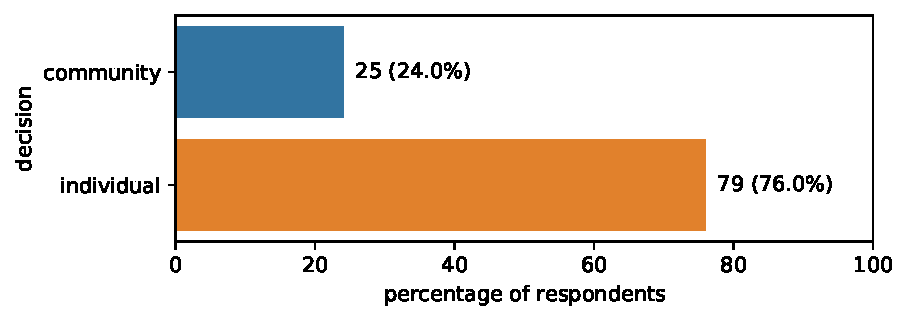
\includegraphics[width=1\columnwidth]{pdfs/decision.pdf}
        \label{fig:decision}}
    \hfill
    \subfigure[What was the motivation for creating the variant of the mainline project?]{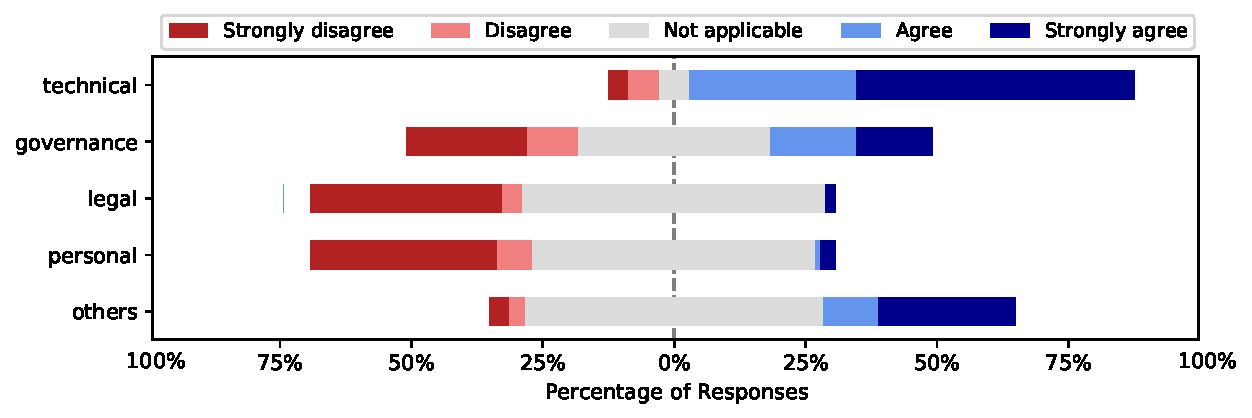
\includegraphics[width=1\columnwidth]{pdfs/likert_motivations_1.pdf}
    \label{fig:motivations}}
    \hfill
    \caption{\RQOne}
     \label{fig:decision_motivations}
     \vspace{-.3cm}
\end{figure*}

\section{\RQOne}
\label{sec:results-RQ1}
RQ1 aims to investigate whether new motivations for creating variant forks have changed since the advent of social coding platforms. To do so, we asked the survey participants the following questions:

%\begin{itemize}
%\item
 \rqOneOne

%\item
 \rqOneTwo

%\item
\rqOneThree
%\end{itemize}


% We now presents and analyses the results of the survey.
% In some cases we quote the survey respondents using [R$N$] to refer to a quote coming from respondent numbered $N$.

For $SQ^1_{a}$, we presented a multiple choice question. In $SQ^1_{b}$ we presented Likert scale answer options, while $SQ^1_{c}$ was an optional open-ended question. For the latter, we coded the respondent's answers into themes and categorised common responses.
When quoting the survey respondents, we refer to them using [R$N$] notation, where $N$ is the respondent's ID.
%\sd{this is kind of redundant with what came earlier}
The respondents' answers that include the selection on the multiple choice answers as well as the themes resulting from coding open-ended answers are \dashuline{underlined}.
The open-ended responses are presented in \emph{italics}.
Where applicable, we integrate and compare our findings with related research findings.

\subsection{Results}
Fig.~\ref{fig:decision_motivations} summarises the responses for $SQ^1_{a}$ and $SQ^1_{b}$. Fig.~\ref{fig:decision} shows that the majority of the participants responded that the decision was \dashuline{individual}. Fig.~\ref{fig:motivations} shows that the majority ranked highly the \dashuline{technical} motivation for creating variants. We also see quite a number of highly ranked motivations of \dashuline{governance} and \dashuline{others}.
% Like we presented in Section~\ref{sec:protocal}, th
% is question had Likert scale answer options we identified in the literature. 2) \emph{Was the motivation for creating the variant an individual decision or a community decision?} This survey question had two multiple choice answers of: \emph{individual} or \emph{community} decision.

While previous studies have investigated the motivations for creating variants, no study has investigated the details of those motivations ($SQ^1_{c}$) .
To identify these details, we proposed two optional open-ended questions to allow the respondents to provide details on their Likert scale answer to $SQ^1_{b}$. The two questions were
(1) \emph{Kindly provide details for your selected answer(s) on the motivation;}
and (2) \emph{If there are any links that are documented relating to your choice of answers on motivation detail, kindly point us there}.

100 of the 105 survey respondents\tm{Incorrect, there were 112 respondents according to section II.C!}  provided details of their motivation for creating a variant fork, and 30 of the 100 provided with extra pointers.
The coding process for the open-ended question (see Section~\ref{sec:card_sorting}), allowed us to identify the five missing details of the choice of motivation\tm{I do not understand what you mean by the "five missing details". Why five and what are you referring to exactly?} by looking at selected response as well as comparing contents of the mainline and variant repositories on \gh.

Fig~\ref{fig:sankey_motivation} presents a Sankey diagram summarising the details of the respondents' choice of motivation based on the coded themes. 
The figure  presents the distribution of the responses to all questions relating to $RQ1$ and how these responses relate to each other. The thickness of the edge represents the frequency of respondents between two entities.
%The axis--\texttt{variant status} in Fig~\ref{fig:sankey_motivation} shows the variants that are attached to- or detached from the mainline repository as discussed in Section~\ref{sec:forks_and_participants}.

Focusing on the axes of \dashuline{decision} and \dashuline{motivation}, we can confirm the observations from Fig.~\ref{fig:motivations} that the majority of respondents had an \dashuline{individual} and \dashuline{technical} motivation.
The majority of respondents that answered the question \dashuline{original developers?} selected \dashuline{none} implying that the majority of the variants were started by different developers.
Since the answers to $SQ^1_{c}$ were presented on a Likert scale,\tm{This seems incorrect,since SQ1c is open ended. Do you mean SQ1b perhaps?} participants were asked to rank the appropriate motivation(s) to why they created the variant. While coding the motivations details, we identified respondents who ranked highly more than one motivation category and also provided a response in the open-ended question to support each highly ranked motivation category. In this scenario, eachhighly ranked motivation category would have a motivation detail for the same respondent. %\az{I added the following information and modified the text introducing each motivation (detail)}
At the end we found that 105 of the survey participants chose 145 motivation categories, of which 84 \dashuline{technical}, 34 \dashuline{governance}, 3 \dashuline{legal} and 24 \dashuline{others}. Below we present the common motivation themes and some  specific responses we found very
interesting.

\begin{figure*}[ht]
\begin{center}
    \centering
    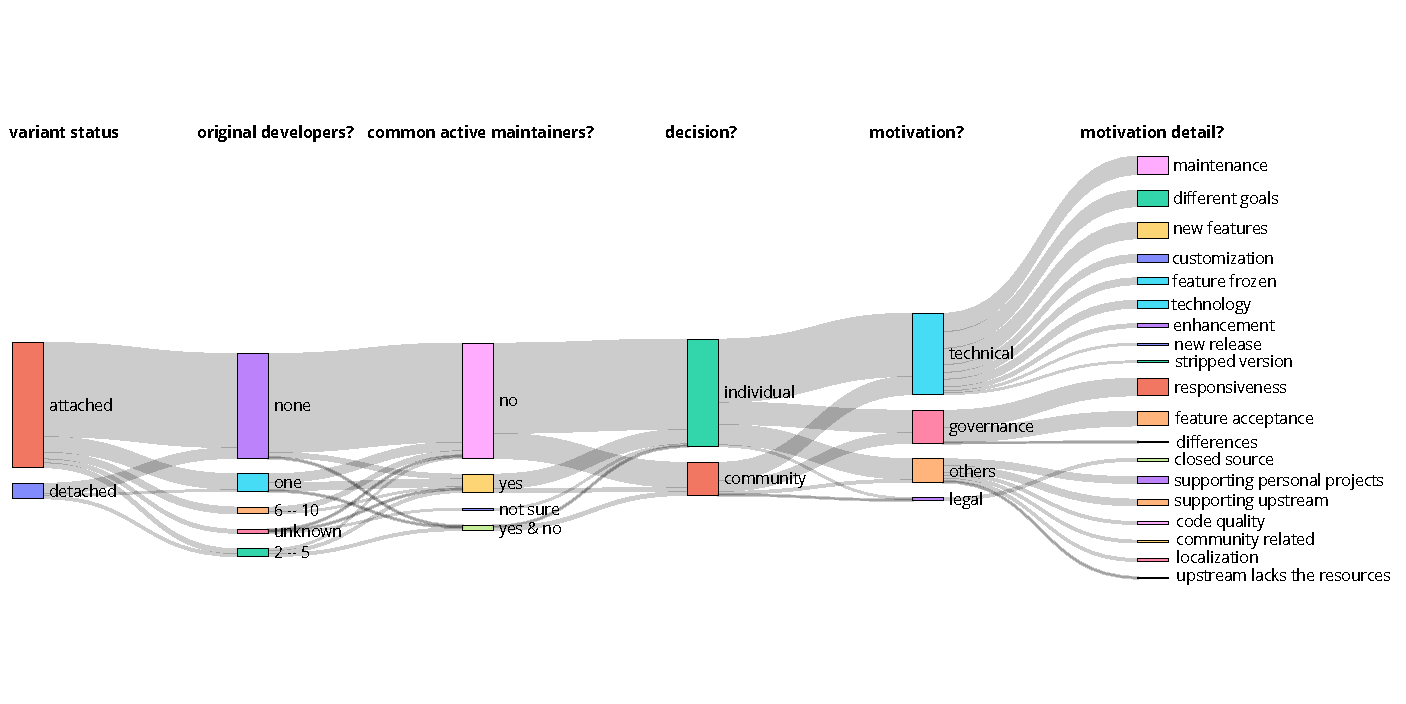
\includegraphics[width=\textwidth]{pdfs/sankey_motivations_2.pdf}
    \caption{Sankey diagram summarising the detailed motivations behind creating variant forks.
    }
    \label{fig:sankey_motivation}
\end{center}
\vspace{-.3cm}
\end{figure*}

\nd \textbf{Technical.} \dashuline{maintenance} is the most frequent motivation detail for the \dashuline{technical} motivation. 19 of the 84 survey participants who selected \dashuline{technical}, mentioned phrases related to \emph{performing bug/security fixes}.

\begin{itemize}[leftmargin=*]

%\item \emph{The fork was created because that is how you contribute changes back to a project on github, then the original maintainer of the project abandoned it making my fork the main actively developed one} [R38]. %This motivation detail can be related to the findings of Robles and Gonz{\'a}lez-Barahona~\cite{Gregorio:2012} who reported that one of the outcomes of forking is

\item ``\emph{The PR to merge the fork's new capabilities into the mainline code was too large, [...] %resulting in a long review time,
and my attempts to incorporate feedback into the PR [...] %(using force-pushes that disrupted the review process)
ended upsetting the primary maintainer who has been studiously ignoring the pull request for three years \frownie{}}'' [R59].
This respondent ranked highly both \dashuline{technical} and \dashuline{governance}. The respondent also provided a \gh link to their pull request to the mainline. Indeed, we found that the pull request was made in February 2018 and received 218 comments from both the mainline maintainer and the respondent discussing its details. On October 2021, the pull request is still open.

\item ``\emph{I forked the original project in order to fix a bug. However, the way the original was architected made this very challenging, so I ended up rewriting it instead of submitting a patch to the original}'' [R79].

%\item ``\emph{The original project did not take WCAG accessibility guidelines into account. We first tried to make improvements on it, but they were broken soon after. So we finally decided to fork the project with the explicit aim to focus on accessibility}'' [R88]. A \gh issue link provided by the respondent showed that the question ``\textit{Did this start as an experiment or an intentional hard fork?}" was explicitly asked to the variant maintainers. The latter responded by mentioning that at first their intention was to improve the mainline and not maintain a different project, but later, some of their merged fixes were removed from the mainline. This led them continue maintaining their fork in a different way.
%\ad{That one seems more a ``different goal''.}\jb{I agree}\az{I am not sure if it different goals. Check my text above and https://github.com/KIProtect/klaro/pull/39}

\end{itemize}

\nd The next prominent \dashuline{technical} motivation detail was \dashuline{different goals}. 17 of the participants who selected \dashuline{technical}, mentioned phrases related to \emph{variants present different goals\,/\,content\,/\,communities\,/\,directions}.

\begin{itemize}[leftmargin=*]
\item ``\emph{[We] %Difference in content -
list websites that accept Bitcoin Cash cryptocurrency, as opposed to the mainline that lists websites with 2 factor authentication}'' [R1].
\item ``\emph{The original goal of the mainline is completely different from the fork variant. % While the projects are related in the sense that they share a similar code base, they are very different pieces of software
}'' [R4].
%\item ``\emph{This is a cryptocurrency, which introduced a completely different monetary policy, and consensus, while keeping many of the original features of the mainline. It is worth noting that [...] %, for the same principle, the mainline itself is a variant of another project% (bitcoin/bitcoin)}'' [R70].\az{we gave enough examples here)}
\item  ``\emph{We wanted to take the project in a different direction}'' [R100].
\end{itemize}

\nd The next prominent \dashuline{technical} motivation detail was \dashuline{new features}.
17 of the participants who selected \dashuline{technical}, mentioned phrases related to \emph{introduction of new features not in the mainline}.

\begin{itemize}[leftmargin=*]
\item ``\emph{[...] to add support for a feature I knew would not get merged into the main project}'' [R53].
\item ``\emph{Mainline developer only does bugfixes and eventual underlying runtime/SDK upgrades to stay current. He did not add new features due to lack of interest \ldots}'' [R67]
%\ad{This one better fits in ``feature frozen''}
%\jb{}
\item ``\emph{Our variant introduces new experimental functionality that is not yet ready for use in the mainline}'' [R80].
\end{itemize}

\nd The next prominent \dashuline{technical} motivation detail was \dashuline{customization}.
8 of the participants who selected \dashuline{technical}, mentioned phrases related to \emph{variant customizes the mainline features}.

\begin{itemize}[leftmargin=*]
\item ``\emph{The ``bones'' were good, but I wanted to add some aesthetics [...] %. Given the original prided itself on minimalism, it didn't feel right to contribute it into mainline.
so, I forked it to make it pretty and my own}'' [R10].
%\ad{Check the above quote. I removed an interesting part (``it didn't feel right to contribute it into mainline''). If you decide to keep it, then I suggest to move this quote to the ``different goals'' category.}
\item ``\emph{The new version is a vectorized, accelerated version of the original.%, but used some common code. It's not so much a fork as ``inspired by'', but we wanted to give due credit
}'' [R37].
\item ``\emph{[We] added some syntactic sugar and some improvements by itself \ldots}'' [R42].
%\ad{This last one would better fit in ``no longer maintained''.}
\end{itemize}

\nd The next prominent \dashuline{technical} motivation detail was \dashuline{unmaintained feature}.
%\sd{Every paragraph starts with ``The next prominent \ldots". This quickly gets repetitive. I am also not sure whether you should include them all. If you need to cut space, here is one place where you may do it.}
8 of the participants who selected \dashuline{technical}, mentioned phrases related to \emph{one of the mainline feature used by the variant is no longer maintained}.
%\ad{I don't get the link between ``feature frozen'' and ``feature no longer maintained''. You can freeze a feature while maintaining it (e.g. by providing patches or improvements to it). I suggest to rephrase it to ``unmaintained feature''.}

\begin{itemize}[leftmargin=*]
\item ``\emph{The `shiny' component of mainline was declared to be no longer maintained around the time I created our fork. [\ldots] I did not like many of the architectural decisions of the original project, I opted to create a fork instead of volunteer to maintain the original.}'' [R65]. The respondent provided an extra link. An issue about `shiny' component was opened up in Jul 2015 and closed in Jul 2017. The issue contained 93 comments from 35 participants. When closing the issue the maintained stated that ``\textit{[...] If somebody or bodies from the community wants to fork the source code and run with it, they have my blessing [...]})''. The variant was created on Aug 2017.
%\ad{This one fits in ``new technology''.}
\item ``\emph{The mainline project had made a radical shift from providing one set of features %(pip-review + pip-dump)
to a different, disjoint set of features. % (pip-compile + pip-sync).
The maintainer had thought about it very well, but some users (including myself) had built their workflows around one of the old features. For this reason, I lifted that particular feature into a separate project that was also published under a different name to the package index.%For these historical reasons, the mainline and the variant are not really alternatives to each other; rather, they are complementary
}'' [R23]. The respondent also provided us a link, \gh \texttt{issue}, discussing the details. The \texttt{issue} was opened by the variant maintainer on July 2015 and was eventually closed on April 2018. The \texttt{issue} had 33 comments involving 17 participants. %\jb{need to link with other qns}.
%\ad{@John: I like this kind of ``anecdotal evidences'', but I'm missing how it contributes to the point. Also, there should be something wrong about the dates, since it means the issue was closed before its opening.}

\item ``\textit{Mainline dropped support for a small subset of the code and asked for community support to create a fork to support that subset}'' [R66].
%\ad{If a set of features is dropped, doesn't that mean the projects went into different directions? It's not only ``we do no want to maintain this feature'' but rather ``we removed it, if you need it, do your own project''. If I'm right, this means it better fits in the ``different goals'' or in ``new features'' category.}
\end{itemize}

\nd The next prominent \dashuline{technical} motivation detail was \dashuline{technology}.
7 of the participants who selected \dashuline{technical}, mentioned phrases related to \emph{variant created to depend on a different technology}.

\begin{itemize}[leftmargin=*]
\item ``\emph{Added support for Open Street Maps as an available map provider [\ldots] mainline was not willing to accept this kind of contribution.}'' [R8]. This was also ranked as a \dashuline{governance}.
\item ``\emph{The mainline wasn't updated to use .NET Core which I was using in my project, so I updated it}'' [R29].
\item ``\emph{[...] to keep the source code compatible with the language/compiler version that we use (Swift / Xcode). [...] %Sometimes new versions of Swift break source compatibility, if we update (or not update when there is a new one) the compiler but
if the maintainer of the mainline is supporting a different one, then we could not compile our dependency anymore}'' [R54].
\end{itemize}

\nd \textbf{Governance}. The motivation of \dashuline{governance} is connected to the second most motivation details mentions, with the most prominent being \dashuline{responsiveness}. 18 of the 34 survey participants who selected \dashuline{governance}, mentioned phrases related to \emph{mainline was unresponsive to pull requests or issues for a long time}. Most of the respondents that ranked highly \dashuline{governance} as the motivation, also ranked highly other options of motivations. Only 4 of the 34 ranked only \dashuline{governance}.

%\ad{Very first quote seems to belong to this category}

\begin{itemize}[leftmargin=*]
\item ``\emph{[They] %The parent repo
had a series of commits that fixed functionality for newer PHP versions, but never made into a release. %The library was being used in an enterprise app using Composer/Packagist, which requires a new GitHub release to update the published library.
After waiting for more than a year for a release, a fork was done just to push a newer release into Composer/Packagist}'' [R21].

\item ``\emph{We submitted some bug fixes [...], %to the original repo
but didn't hear back from the maintainer for a while and needed to progress to meet our own goals so we forked. I followed up over email with the maintainer and he merged the patches about a month later, at which point we closed down and archived our fork and returned to using the mainline}'' [R15].
Merging back to the original corresponds to one the outcomes of variant forking reported by Robles and Gonz{\'a}lez-Barahona~\cite{Gregorio:2012}.
%\ad{That one suggests we wrongly identified the variant fork (since it has been active for only one month). I suggest to remove this quote.}

\item ``\emph{%\ldots created in order to submit PR into mainline. Its purpose has changed
[...] due to lack of response from mainline maintainer (more than months) and need of release. This lead to release of a new variant. [...] there is no intention to submit changes to mainline anymore (even when the first PR was merged into mainline after more than year)}'' [R56].
\end{itemize}

\nd The next prominent \dashuline{governance} motivation detail was \dashuline{feature acceptance}.
15 of the participants who selected \dashuline{governance}, mentioned phrases related to \emph{mainline hesitant to or not willing to accept feature}.

\begin{itemize}[leftmargin=*]
\item \emph{``TECHNICAL: Added support for Open Street Maps as an available map provider. GOVERNANCE: not exactly governance, but mainline was not willing to accept this kind of contribution"} [R8]. This was coded as \dashuline{technology} in \dashuline{technical}. The respondent also provided a \gh pull request link that contains extra information, that we examined. The pull request contained 45 conversations and 15 participants between June 2018 until March 2021 when it was closed.
%\ad{I suggest to remove this quote since it combines two distinct reasons, and we do not explain that a respondent could select more than one reason (and what we did when they did).}

\item ``\emph{Mainline was not ready to accept those changes in part because the maintainers were not responsive. Since that time all of the issues have been dealt with and my variant is no longer needed, though the infrastructure for creating a new release of the variant remains in place in the event that it might be needed in the future}'' [R44].

\item ``\emph{%Yes, there were attempts, but at then end
[...] even main repo maintainer was saying he is busy and please use your fork for thing X and Y. We don't know the exact reason why he stopped maintaining it and also did not allow us to maintain his repo}'' [R89]. In one of the multiple choice answers, the respondent indicated that the variant was created through a  \dashuline{community decision}.
The respondent also provided an extra link, in which we discovered that
%The respondent also provided extra links (two issues on the mainline) relating to the motivation of creating\,/\,maintaining the variant.
% we found that the variant was created through a \dashuline{community decision}.
%In the issues the extra links,
three contributors from the community were interested in a couple of new features that were missing in mainline, but the mainline maintainer seemed busy. At the end, two members of the community took over the fork maintenance and introduced the missing features and advertised the additions in the \textsf{readme.md} file of the fork as well as in the issue.

\end{itemize}


\nd \textbf{Others}. %The motivation of \dashuline{others} is connected to the second\az{I don't understand this. I will modify the text} most motivation details mentions, with the most prominent being \dashuline{supporting personal projects}.
The most prominent motivation detail for \dashuline{others} motivation is  \dashuline{supporting personal projects}. 8 of the 24 survey participants who selected \dashuline{others}, mentioned phrases related to \emph{variant was created to support personal projects}.


\begin{itemize}[leftmargin=*]

\item ``\emph{%Fairly boring as it's a very small library.
[The] maintainer %of the ``mother'' repo
was not interested in a PR that added functionality needed by a project I'm developing. [It] was considerably easier to add the logic into the [new] library than bolt it on.%, so I forked the library
}'' [R18]. This was ranked as \dashuline{technical}, \dashuline{governance}, and \dashuline{others}. As we can see in the participant response we have phrases like ``\textit{adding logic}" (\dashuline{new features, technical}), ``\textit{was not interested in a PR}'' (\dashuline{feature acceptance, governance}), and ``\textit{functionality needed by a project I'm developing}'' (\dashuline{supporting personal projects, others}).

\item ``\emph{In Oct 2017 Twitch.TV has changed its API and these changes broke the mainline project. I used this project daily and needed to fix it ASAP. After quick fix I started to add my own features. [...] the mainline project has been fixed and refactored, but my other projects were already depending on my own fork}'' [R56].

\item ``\emph{%The main reason for forking (OTHER) is
[...] to make sure that no matter what happen to the mainline repository, we can maintain source access to this library, which is an essential dependency of our project. \ldots}'' [R54]. This response is inline with the findings of Nyman et al.~\cite{Linus:2012Perspectives} who reported that forking provides a mechanism for safeguarding against despotic decisions by the project lead, who is thus guided in their actions to consider the best interest of the community.

\end{itemize}

\nd The next prominent \dashuline{others} motivation detail was \dashuline{supporting mainline}.
7 of the participants who selected \dashuline{others}, mentioned phrases related to \emph{supporting mainline}.
%\ad{So far, my impression is that we already have many cases of mainline maintainers hesistant to or not willing to accept feature spread in the above categories, for some reasons. I don't really get what is different here.}

\begin{itemize}[leftmargin=*]
\item ``\emph{We have a fork that is the ``main fork'', which is eclipse, and the ``development fork'' is OpenTOSCA. In this case, our modling tool [\ldots] is only maintained as the fork [\ldots] we synchronize everything between both forks while the OpenTOSCA one is mainly used to develop new features, which are then pushed as PRs to the main fork}'' [R61].
%\ad{This seems like a social fork, mostly for PRs, but at a different level than the usual social fork.}

\item ``\emph{Preparation of mainline pull requests. mainline repo should not be spammed by WIP PRs by students. Supervisors do coaching and try to improve the quality by the initial mainline pull request. [\dots] Keeping the PR open on the fork, reduces the number of PRs}'' [R73].
%\ad{Same here.}

\item ``\emph{We needed a repository for tracking our ideas to keep the number of issues of the main repository low}'' [R83]. An extra link was provided, in which we found that the mainline and variant are owned by the same developer: ``\emph{this repository is used by [X] to make his ideas transparent. He collects the issues here to avoid flooding the ``official'' issue tracker. - Refined issues will be migrated to the official issue tracker}".
%\ad{This last example confirms that this last category is not well defined. It's not about ``mainline hesistant to or not willing to accept feature'' but rather to prevent the mainline to be flooded by students' PRs, attempts, etc.}
\end{itemize}

\nd The next prominent \dashuline{others} motivation detail was \dashuline{code quality}.
3 of the participants who selected \dashuline{others}, mentioned phrases related to \emph{mainline low code quality}.

\begin{itemize}[leftmargin=*]
\item ``\emph{%The main reason I forked was code-quality.
The mainline [...] % library works, but
was clearly written by someone who isn't a professional software engineer.% Also: mainline was not properly packaged (and still isn't AFAIK).
}'' [R63].

\item ``\emph{%I forked the original project in order to fix a bug. However,
The way the original was architected made this very challenging, so I ended up rewriting it instead of submitting a patch to the original}'' [R79].
\end{itemize}


\nd \textbf{Legal}. The motivation of \dashuline{legal} is connected to the least number of motivation details mentions, with the most prominent being \dashuline{responsiveness}. It had only 3 of the 105 survey participants that indicated phrases related to \dashuline{closed source}. Below we present their corresponding responses.
%\ad{I see three items. Do we have 3 ``most interesting responses'', or 3 excerpts from 2 responses?}

\begin{itemize}[leftmargin=*]
\item ``\emph{[The] main reason is creating [an] open source and commercial product which has much more features% and we just collect open source components and use them. Red5 server is one of the component of the product
}'' [R7]. This motivation detail was also categorised as: \dashuline{(new features, technical)} and \dashuline{(supporting personal projects, others)}.

\item ``\emph{5 years ago the permissions model for GitHub and Travis is not what it is today. I wanted to use Travis but if I granted Travis access to my primary github account, it would have read access to all the github repos [...], which would expose private customer code. I forked the repo [but] the permissions model has evolved [and I] %I have a pending task to switch to github actions for CI/CD on the main repo, and to
deleted the fork}'' [R24].

\item ``\emph{The founders of the mainline had been absent from the project for several years, but came back and booted the maintainers off and
[...] shifted the project to a closed source. %There was an attempt to reconcile differences [...], but the these issues were resolved (at least from the point of view of the maintainers, in reality the founders just pretended to be fine with it and secretly plotted for the next year to remove the maintainers from the project and ban them from every community to minimize a potential fork when they announced their plans to change the license
}'' [R36]. %The decision to create the fork was initiated by the \dashuline{closed source}.
%Ahmed: I commented the text below because I don't see its added value.
The respondent provided a link with extra information showing that three of the maintainers that were booted from the original project and a fourth one from the community joined forces and are now maintaining the variant. The variant currently has over 739 stars, is used by 35 developers, has 101 pull requests and 195 issues.
\end{itemize}


\subsection{Discussion and Implications}
In this study we were mainly interested in finding out the motivations for creating and maintaining variants especially those that actively being maintained in parallel with their mainline counterparts.
We have identified that the decision to create the variants is mostly initiated by individuals and less by community.
Our findings here confirm the findings in the literature.
% The survey participants revealed that they created variants for technical, governance, legal reasons that are reported in literature.
Our study also extends the findings in literature by providing fine-grained reasons for creating and maintaining variants relating to the previously reported reasons.
Furthermore, our study has also revealed other reasons not listed in literature that respondents categorised as \dashuline{others}, which include: 1) supporting the mainline, 2) variant supporting other personal projects, 3) localization purposes and 4) variants developers not trusting the code quality of the mainline.
The findings reported here will be very useful in follow-up studies in investigating the co-evolution of mainline and variants.

In Fig.~\ref{fig:sankey_motivation} we also present an overview of how the detailed motivations relate to who is involved in creating and maintaining the variants. We can see that the motivations majorly relate to developers outside (82\%) the core contributors of the mainlines. We also observe quite a significant (24\%) number of respondents indicating that the decision to create the variant was initiated by the community. We have also observed from the open-ended responses, that before the transition from social to variant fork, some variant maintainers engage with the mainline maintainers through discussions in issues and pull requests. This is inline with the findings of Zhou et al. who reported that many variant forks start as social forks~\cite{Zhou:2020}

Besides the motivations for creating and maintaining of variants, the respondents have reported some interesting software reuse practices by the variants, like those categorized in the themes of: \dashuline{different goals}, \dashuline{new features}, \dashuline{customization}, \dashuline{technology}, \dashuline{supporting personal projects}, \dashuline{supporting upstream}, \dashuline{localization}. A specific example of [R70] categorized in the \dashuline{different goals} theme, stated that in the cryptocurrency world, all applications inherit code from the mother project \textsf{bitcoin/bitcoin}. Downstream applications also monitor their immediate upstream and other in the hierarchy for important updates like bug and security fixes as well as other specific updates. These cryptocurrency applications can be considered as a \textit{software family}~\cite{businge:2018icsme,businge:emse:2021}), that are part of dedicated project ecosystem~\cite{tommens:2020}, continuously reuse code among themselves.
There are other dedicated software ecosystems that exist like, \textsf{Eclipse}, \textsf{Atom}, and \textsf{Emacs}, programming language ecosystems like:  \java, \cp, \cpp, \py, \go, \rb, operating system ecosystems like: \textsf{macOS}, \textsf{Linux}, \textsf{Windows}, and \textsf{iOS}~\cite{tommens:2020} can contain variants.
To this end, our study opens up different research directions that can be aimed at deeply investigating these different reuse practices in \textit{software family} and software variants in general. A deeper understanding of these reuse practices can aid the development of tools that can support more efficient software reuse.

\begin{custombox}
\emph{\textbf{Summary -- RQ1}:
Many variant forks start as social forks. The decision to create\,/\,maintain the forks is either community-driven (contributing up to 24\%) or individual (76\%). The majority  of the developers (82\%) creating the forks are not maintainers of the mainlines. We have presented 18 variant creation\,/\,maintenance motivation details categorized in the motivations of \dashuline{technical} (accounting 58\% of the responses), \dashuline{governance} (24\%), \dashuline{others} (16\%) and \dashuline{legal} (2\%). The detailed motivations in the \dashuline{others} category are newly introduced in the social coding era.
% Ahmed: text below could be added to introduction/conclusion/abstract
%We have also discussed some interesting software reuse classifications among variants.
}
\end{custombox}


\begin{figure*}[ht]
\centering
\vspace{-.3cm}
    \hfill
        \subfigure[$SQ^2_{a}$. How many mainline developers involved in creation of variant?]{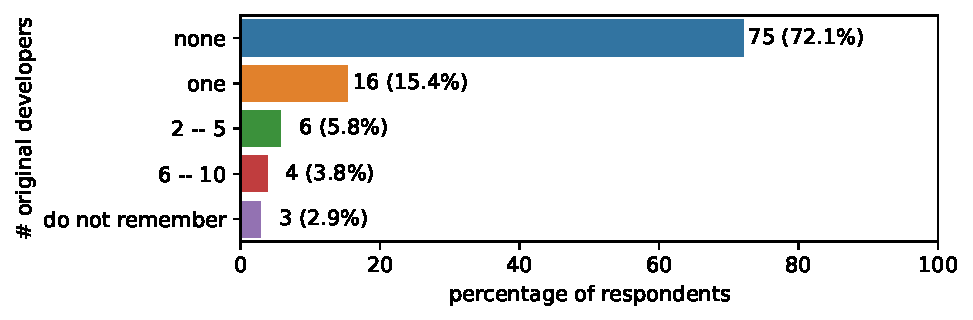
\includegraphics[width=1\columnwidth]{pdfs/original_developers.pdf}
        \label{fig:original}}
    \hfill
    \subfigure[$SQ^2_{b}$. How many common active maintainers are there between mainline and variant?]{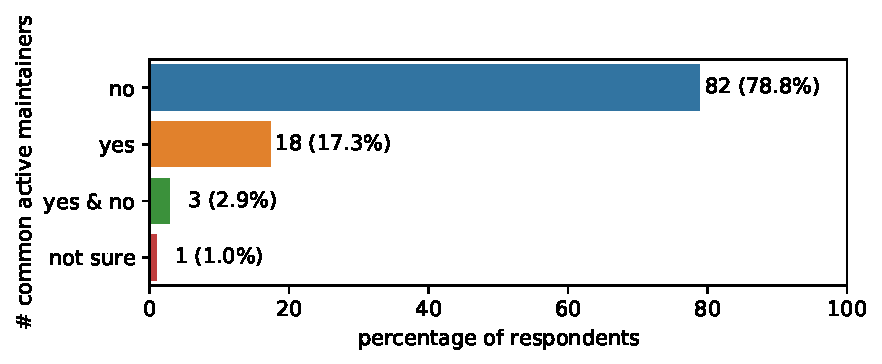
\includegraphics[width=1\columnwidth]{pdfs/common_maintainers.pdf}
    \label{fig:common}}
    \hfill
    \caption{Who are the developers involved in creating and maintaining variants of a mainline project?}
     \label{fig:original_common}
     \vspace{-.3cm}
\end{figure*}



\section{\RQTwo}
\label{sec:results-RQ2}
%Recall that in Section~\ref{sec:intro} we stated
$RQ2$ aims  to identify the impediments for co-evolution between the mainline and variant projects.
This question lead to two specific survey reflecting the \textit{who} and the \textit{how}, respectively. The \textit{who} aimed at identifying the developers involved in maintaining these variants. The \textit{how} aimed to understand how variant  projects evolve  w.r.t. the  mainline.
As for $RQ1$ we refer to the responses using \dashuline{underlined}, \emph{italics} and [R$N$].



\subsection{Results for the ``\emph{who}'' question}
To answer the ``\emph{who}'', we asked the following 2 questions:

%\begin{itemize}
%\item
 \noindent \rqTwoOne

%\item
\noindent \rqTwoTwo
%\end{itemize}

For both $SQ^2_{a}$ and $SQ^2_{b}$ we provided multiple choice answers to the questions. We present the results of $SQ^2_{a}$ and $SQ^2_{b}$ in Fig.~\ref{fig:original_common}. Looking at both Fig.~\ref{fig:original} and Fig.~\ref{fig:common} for both questions respectively, we can see that the majority of the participants chose the options of \dashuline{none} (none of the creators of the variant were part of the mainline) and \dashuline{no} (they do not have common active maintainers).
This implies that most of developers that are involved in the creation and maintenance of the variants are outside the core maintainers of the original project from where the variant was forked.
The difference in the numbers of participants who selected  \dashuline{none} for $SQ^2_{a}$ and \dashuline{no} for $SQ^2_{b}$ can be visualized in Fig.~\ref{fig:sankey_motivation}.
When we look at how responses of $SQ^2_{a}$--\dashuline{original developers?} and $SQ^2_{b}$--\dashuline{common active maintainers?} are associated, we can see that the majority of the respondents that selected the option \dashuline{none} in $SQ^2_{b}$ went ahead to select the option \dashuline{no} in $SQ^2_{a}$. We can also see other associations between all responses of $SQ^2_{a}$ and $SQ^2_{a}$.
For example, in $SQ^2_{a}$, the participant [R36] who selected the answer option \dashuline{6 -- 10} developers from the mainline were involved in the creation of the variant, also selected the option \dashuline{yes \emph{\&} no} --\emph{``They used to have common maintainers in the early stages of the variant, but now the projects have technically diverged away from each other, there are no more common maintainers"} in $SQ^2_{b}$.
We also observed that respondents [R51] and [R57] who selected the option \dashuline{6 -- 10} and \dashuline{2 -- 5}, respectively, for $SQ^2_{a}$ also selected the option \dashuline{no} for $SQ^2_{b}$. This implies that there were at least two maintainers involved in the creation of the fork, but none of those maintainers is currently contributing to both repositories.



The results of $SQ^2_{a}$ and $SQ^2_{b}$, answer our question on \textit{who is creating and maintaining these variants?} \textbf{Our observation is that the variants are created and maintained by developers different from those in the mainline counterparts.} This observation conquers with the findings of an earlier study by Businge et al.~\cite{businge:emse:2021}.

%As opposed to our exploratory study surveying maintainers of variants, the study of Businge et al.~\cite{businge:emse:2021} was a large scale empirical study on mainline--variant pairs from three software ecosystems. They reported that over 82\% of the 10,979 mainline--variant are owned by different developers. In our study we have also found 82\% of variants are maintained by developers different from those in the mainline.

\subsection{Results for the ``\emph{how}'' question}

To answer the ``\emph{how}'', we asked the following 2 questions:

%\begin{itemize}
%\item
\noindent \rqTwoThree

%\item
\noindent \rqTwoFour
%\end{itemize}


\begin{figure}[ht]
\begin{center}
    \centering
    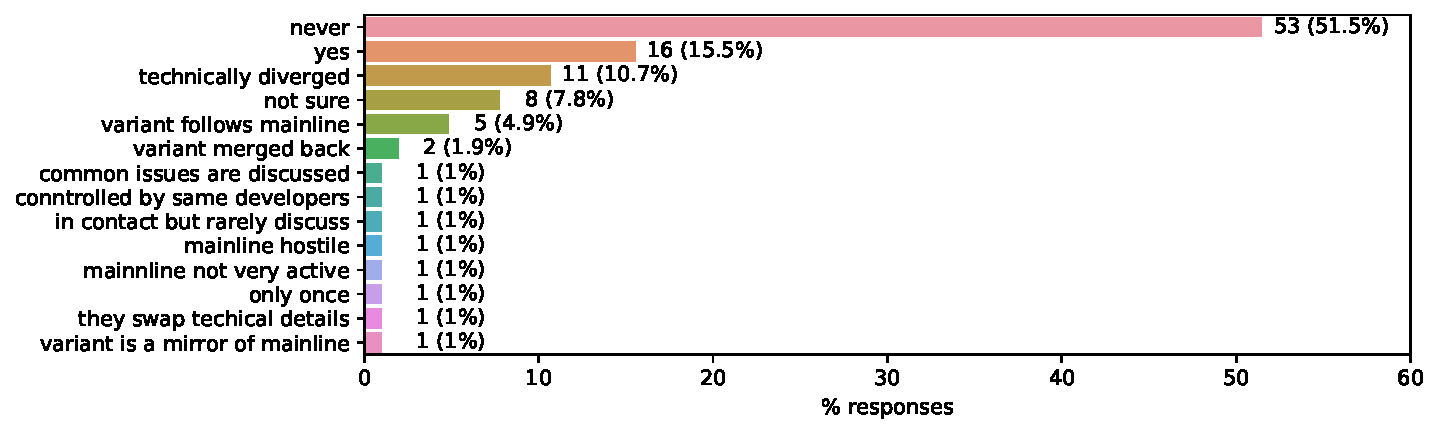
\includegraphics[width=\columnwidth]{pdfs/discussions_rq3_colored.pdf}
    \caption{$SQ^2_{c}$ Do the variant forks and the mainline still discuss the main directions of the project?}
    \label{fig:discussions}
\end{center}
\vspace{-.3cm}
\end{figure}

\nd For $SQ^2_{c}$ we presented four multiple choice answer options. From Fig.~\ref{fig:discussions}, the four answer options we provided for $SQ^2_{c}$ are those with the highest number of responses. We also provided an option of an open-ended answer for participants who felt that their choice is not among the options. The open-ended answers were coded into themes (in Fig.~\ref{fig:discussions} the coded themes are \dashuline{variant follows mainline}\ra to \dashuline{variant is a mirror of the mainline}).
The results in Fig.~\ref{fig:discussions} show that more than 51\% of the responses chose the option of \dashuline{never}--\textit{no, there has never been any discussion since the creation of the variant}. In addition to the participants who selected \dashuline{never}, there are other variants that do not discuss the directions of the project, like \dashuline{mainline hostile} to variant,  \dashuline{not very active},  \dashuline{in contact but rarely discuss}, \dashuline{only once}, and \dashuline{technically diverged}--``\emph{They used to discuss but not anymore since the projects have technically diverged from each other}''.%\az{which [RN]?}

\begin{figure*}[t!]
\centering
\vspace{-.3cm}
    \hfill
        \subfigure[Code integration from mainline]{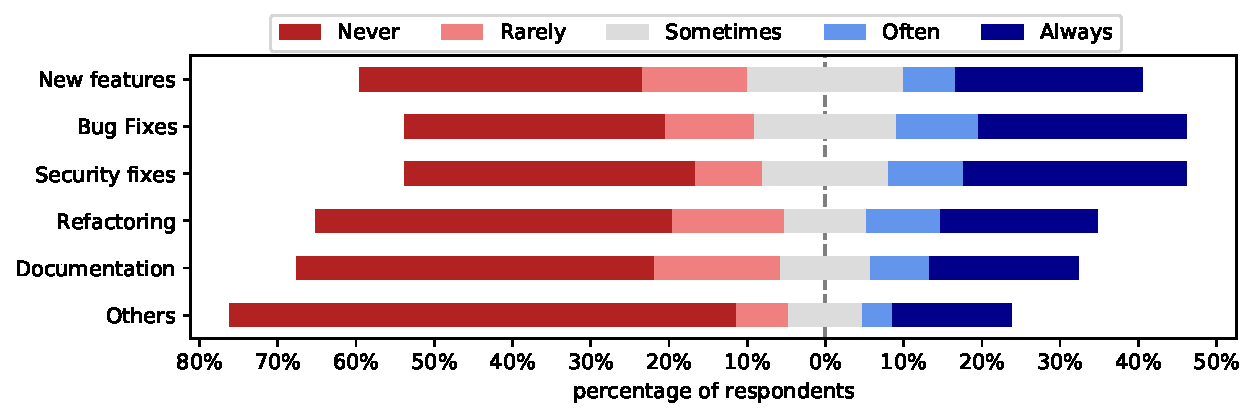
\includegraphics[width=1\columnwidth]{pdfs/likert_integration_from_mainline.pdf}
        \label{fig:from_mainline}}
    \hfill
    \subfigure[Code integration to mainline ]{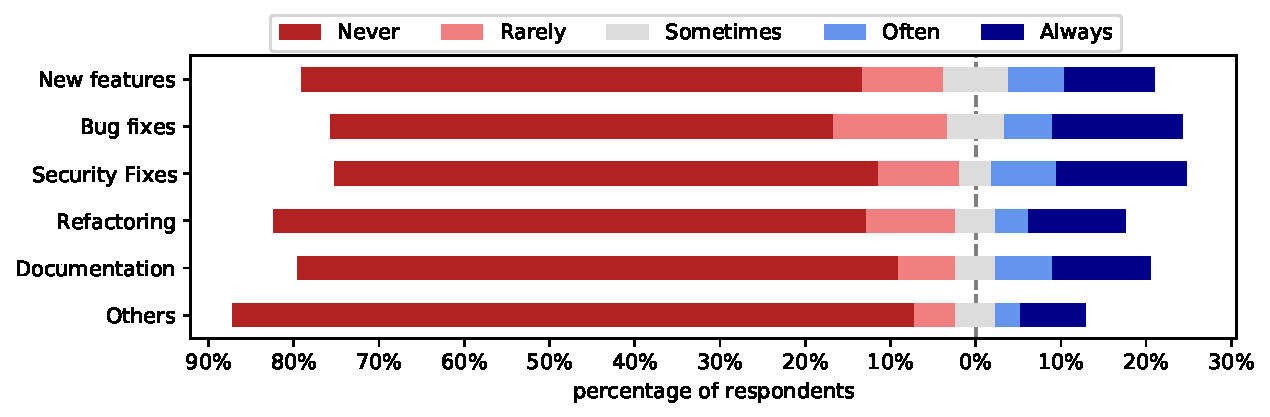
\includegraphics[width=1\columnwidth]{pdfs/likert_integration_to_mainline.pdf}
    \label{fig:to_mainline}}
    \hfill
    \subfigure[integration from mainline (coded themes)]{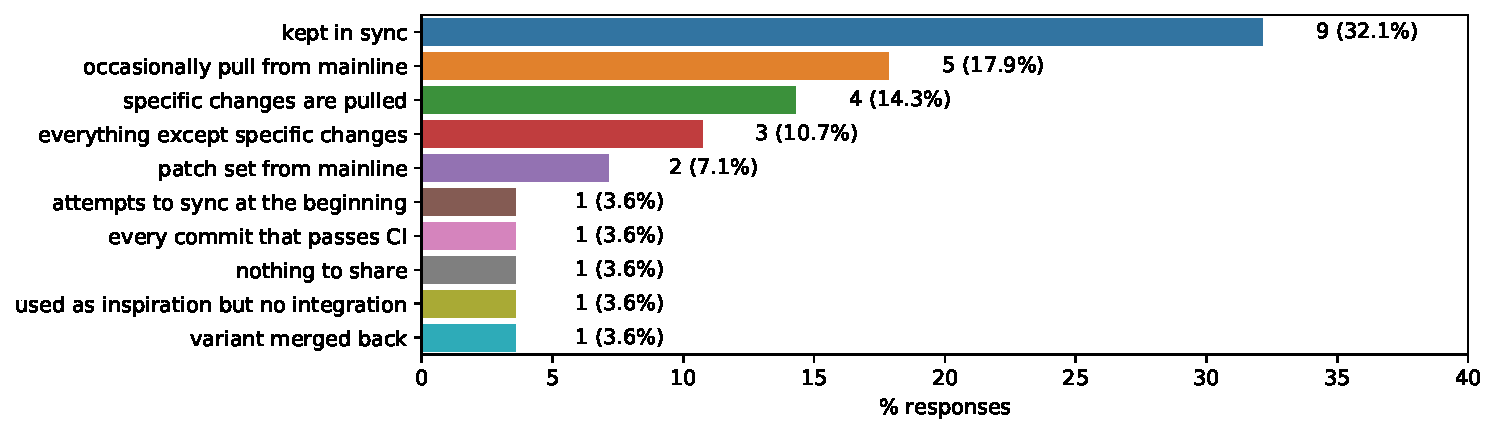
\includegraphics[width=1\columnwidth]{pdfs/changes_from_mainline.pdf}
        \label{fig:from_mainline-coded}}
    \hfill
    \subfigure[integration to mainline (coded themes) ]{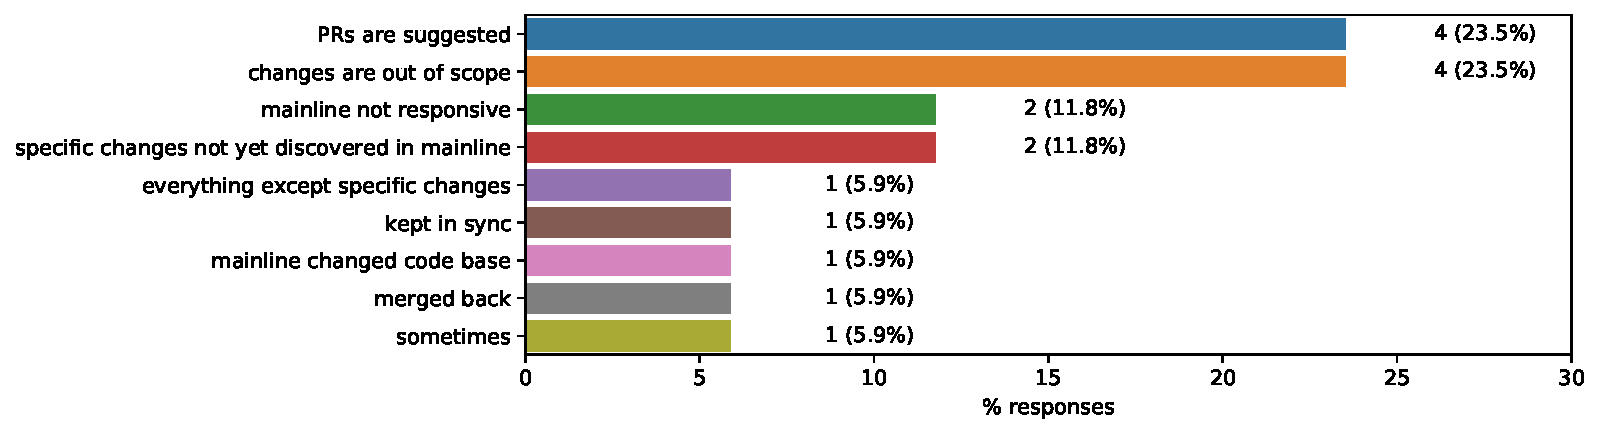
\includegraphics[width=1\columnwidth]{pdfs/changes_to_mainline.pdf}
    \label{fig:to_mainline-coded}}
    \hfill
    \caption{\RQTwo}
     \label{fig:interactions}
     \vspace{-.3cm}
\end{figure*}

An explanation for the high number of variants that do not discuss with the mainline the direction of the projects can be derived from the findings of $SQ^2_{a}$ and $SQ^2_{b}$. The majority of the variants are created and maintained by developers outside the code developers of the mainline. Also, most of the \emph{motivation details} in $RQ1$ could explain the high numbers of \dashuline{never}. For example we have observed that the majority of the variants in the \emph{motivation details} category of \dashuline{different goals}, \dashuline{unmaintained features} in the mainline, those having issues with the mainline \dashuline{responsiveness}, those whose features will not be accepted by the mainline (\dashuline{feature acceptance}), selected  \dashuline{never} in $SQ^2_{c}$. \textbf{To this end, we can conclude that the reasons for the majority of the variants not discussing the directions of the project with the mainlines could be attributed to the range of motivation details for creating the variant as well as the creators of the variants not being part of the core developers of the mainline.}

We found that 5 of the responses indicated phrases related to \dashuline{variant follows mainline}. For example respondent [R77] indicated that ``\emph{in the crypto world, the mainline inherits changes from BITCOIN, for example, security commits, and the variant merges those changes in. So the variant is very interested in every change in the Mainline. However, the variant must maintain the specific new features that we added separately, and the Mainline is not interested in helping the Variant do this.}''
We also observed two interesting cases where the variants merged back to the mainline. This is inline with the findings of Robles and Gonz{\'a}lez-Barahona~\cite{Gregorio:2012} who reported that one of the outcomes of forking is the fork merging back.

In $SQ^2_{d}$, we asked respondents two closed-ended questions:
(1) \textit{How often do the maintainers of the variant integrate the following types of changes from the mainline?}; and (2) \textit{How often do the maintainers of the variant integrate the following types of changes into the mainline?}.
%
We provided Likert scale answers options for the two questions. We also asked the respondents optional follow-up questions with open-ended answers, for each of the two questions, to provide us with extra information.
%In Fig.~\ref{fig:interactions} we present the results of $RQ_{3.2}$.

In Fig.~\ref{fig:from_mainline} we present the results from the respondent answers on what they value most when integrating changes from the mainline. We can see that the highly scored changes are the \dashuline{bug fixes} and the \dashuline{security fixes}. In Fig.~\ref{fig:from_mainline} we can see that most of the respondents were leaning towards the negative side compared to the positive side of the plot.
This implies that most variants are not interested in integrating changes from the mainline.
In Fig.~\ref{fig:to_mainline} we see a similar trend observed in Fig.~\ref{fig:from_mainline}, however, the lean towards the negative side is much more pronounced in Fig.~\ref{fig:to_mainline}.
In Fig.~\ref{fig:from_mainline-coded} and Fig.~\ref{fig:to_mainline-coded} we present the coded themes of the extra information of the open-ended answer questions corresponding to the results in Fig.~\ref{fig:from_mainline} and Fig.~\ref{fig:to_mainline}, respectively. In Fig.~\ref{fig:from_mainline-coded} we present the results of 28 of the participants who provided the extra information, while in Fig.~\ref{fig:to_mainline-coded} we only present the results of 17 participants. This might mean that most variants do not submit changes to the mainline.
In Fig.~\ref{fig:from_mainline-coded} we can see that the most prominent response was related to \dashuline{kept in sync} implying that the variants always keep in sync with the the changes made in the mainline. The next prominent response was related to \dashuline{occasionally pull from mainline} implying that variants from time to time pull changes made in the mainline. Some respondents mentioned phrases related to \dashuline{specific changes are pulled}; for example, [R63] indicated that ``\emph{It's mostly changes that make the library for specific iRobot Roomba models (new ones for example)}''. Other respondents mentioned phrases related to \dashuline{everything except specific changes}; for example, [R48] mentioned that ``\emph{All non-compiler specific changes are pulled}''.
In Fig.~\ref{fig:to_mainline-coded} there were two most prominent answers: \dashuline{PRs are suggested}, for example, ``\textit{Made PRs with changes but those have just been ignored. They're still ``open'' with 0 comments from the mainline dev}'' [R67]. The other prominent answer is \dashuline{changes are out of scope}, for example, ``\emph{We use this as a dependency in another project [\ldots] which is often diverging from the language version of the mainline, so there is little reason for us to push this to mainline}'' [R54]. %Another interesting response is ``\emph{Only compiler non-specific that are discovered \ldots before they are discovered in upstream. [\ldots]}'' [R48].

\subsection{Discussion and Implications}

The results of $RQ2$ revealed that variants are created and maintained my developers outside the core developers of the mainlines.
We have also observed that there is limited interaction between the mainline and variant.
Although we find there is little code integration, the integration from mainline\ra variant is more than that from variant\ra mainline.
Our study confirms and extends the findings of Businge et al.~\cite{businge:emse:2021}: we provide concrete reasons relating to little integration between the mainline and variants that include: 1) \textit{technical divergency}: where variants and mainlines are offering different goals, implementing different technologies, variant is maintaining a part of the mainline that is frozen. 2) \textit{governance disputes}: mainlines are unresponsive to pull requests and issues from the variants and  mainlines not willing or hesitant to accept some features from the variants. One respondent also reported that mainline is actively very hostile to variant as a result of mainline changing license to proprietary.
Another possible reason why there is little code integration is because most of the variants are created and maintained by developers outside the core developers of the mainline.
Furthermore, we have observed that a few mainline--variant pairs that integrate code between themselves are mostly interested in patch sets (security fixes and bug fixes).

Although maintenance and collaboration on social coding platforms like \gh have improved through the tooling, especially distributed version
control systems like Git~\cite{Christian:MSR:2012} and transparency mechanisms on social coding platforms~\cite{Laura:2012:CSCW}, these tools are only ideal for social forks which aim to sync all the changes between repositories.
For example, code integration using pull requests and \textsf{git} tools like  \textsf{merge\,/\,rebase} may not be the best when integrating changes in between mainline and variant forks since they involve syncing upstream\,/\,downstream with all changes missing in the current branch.

In this study, we have observed that some variant maintainers are only interested in integrating commits with specific changes.
A suitable integration mechanism would be commit cherry picking since the developers can choose the exact commits they want to integrate.
However, \gh's current setup does not make it easy to identify commits to cherry-pick without digging through the branch's history to identify relevant changes since the last code integration.
Additionally, even though the variants have diverged from their mainlines, we do believe that since they share common code, some of the common code may go through maintenance to perform some bug and security fixing. These mainline--variant repository pairs being maintained by uncommon developers, chances are that these fixes could be missed or they could be fixed at different times by different developers and hence effort duplication.

Our findings can be very useful to code integration tool builders between mainline and variants to prioritise certain categories of mainline--variant pairs by targeting specific changes.
Ideally, a tooling would help identify possibly important fixes in commits and recommend these commits to mainline or variant developers to support a more efficient reuse.
Some promising studies in this direction have focused on providing the mainline with facilities to explore non-integrated changes in forks to find opportunities for reuse~\cite{Ren:2018} and cross-fork change migration~\cite{Ren:2019}. Also more experimental ideas about virtual product-line platforms for unified development of multiple variants of a project~\cite{Antkiewicz:icse:2014,Fischer:saner:2014,Montalvillo:spl:2015,rubin:icse:2013,Stefan:2016:icsme}.

\begin{custombox}
\emph{\textbf{Summary--RQ2}: Mainline and variants do not usually interact during their co-evolution. The lack of interaction could be attributed to a number of reasons that include: (i) technical (i.e., diverging features), where variants and mainlines are offering different goals or implementing different technologies having nothing to share; (ii) governance (i.e., diverging interests), where mainlines are unresponsive to the requests from community and also uninterested in some features suggested by the community; (iii) legal (e.g., diverging licenses), where the mainline variant has changed the license and integration is no longer possible.
As a result of the divergence, it is likely that important updates (like security patches or bug fixes) could be missed or are duplicated.
%Ahmed: text below should placed somewhere else
%We also report interesting interactions that include: integration of only patches, integration of only specific changes, integration that exclude some specific changes and integration only changes that pass CI.
}
\end{custombox}

% !TEX root = 0main.tex
\section{Threats to Validity}

%This study is based on a survey with the stated aim of gaining insights
%in the motivations for creating and maintaining variants on a social coding platform like \gh.
\noindent \textbf{Construct validity}.
The response categories for the closed questions in the survey originated from a thorough literature review.
The questions were carefully phrased to avoid biasing the respondent towards a specific answer. We validated the questions by consulting seven colleagues from three different universities and through trial runs of the survey with seven participants.
%Despite our best efforts, there could be several reasons why our study is limited.
Social desirability bias may also have influenced the answers~\cite{Furnham:1986}. To mitigate this issue, we informed participants that the responses would be anonymous and evaluated in a statistical form.

\noindent \textbf{Internal validity}. We used an open coding process to classify the participants responses received from open-ended questions. The coding process is known to lead to increased processing and categorization capacity at the loss of accuracy of the original response. To alleviate this issue lack of accuracy, we allowed more than one code to be assigned to the same answer.
%While collecting the dataset, in Section~\ref{sec:forks_and_participants} we indicated that we used some restrictive heuristics that could have eliminated some interesting

\noindent \textbf{Generalizability.} Our study is limited to variants of mainline repositories that are hosted on GitHub. We do not claim that our findings generalize to other social coding platforms.
In addition, the set of participants we interviewed corresponds to those who decided to make their e-mail public and who accepted to take part in our study. As such, they are not {\em de facto} representative of all maintainers of variant forks.

\section{Conclusions}
%\sd{The conclusion feels disconnected from the rest of the paper. We should hint back at the ``Why" and ``How" more explicitly. Also use the summaries at the end of the RQ1 to emphasize the findings better. For the moment this reads to much like "We confirmed previous research and made some small but interesting observation". The ``so what'' is still missing here}


Thanks to social coding platforms like \gh, software reuse through forking to create variant projects is on the rise.
We carried out an exploratory study with 105 maintainers of variants, focusing on answering two key research questions:\\
1) \textit{Why do developers create and maintain variants on \gh?}
We observed that the motivations reported by studies carried out in the the pre-\gh era, still hold. We  identified 18 motivation details  for variant creation and maintenance, categorized in the motivations of \emph{technical} (58\% of the responses), \emph{governance} (24\%), \emph{others} (16\%) and \emph{legal} (2\%). Some of these motivations are newly introduced in the social coding era.

\noindent 2) \textit{How do variants projects evolve with respect to the mainlines?}
We have found that there is little interaction between the variants and their mainlines during the co-evolution and reported possible impediments to the lack of interaction. These include: (i) technical (i.e., diverging features), where variants and mainlines are offering different goals or implementing different technologies having nothing to share; (ii) governance (i.e., diverging interests), where mainlines are unresponsive to the requests from community and also uninterested in some features suggested by the community; (iii) legal (e.g., diverging licenses), where the mainline variant has changed the license and integration is no longer possible.

Our findings are very useful to guide follow-up studies in investigating the co-evolution and reuse practices between mainline and variants. A deeper understanding of these practices can aid code integration tool builders in developing tools to support more effective software reuse between mainline projects and their variant forks.

\section*{Acknowledgment}
This work is supported by the joint FWO-Vlaanderen and F.R.S.-FNRS Excellence of Science project SECO-ASSIST under Grant number O.0157.18F- RG43.

%has extended the findings of these previous studies by providing more fine-grained common motivations for creating variants relating to: different goals\,/content\,/communities, customization, supporting personal projects, supporting the upstream, localization, up-taking a unmaintained feature.

%The study also extends the previous studies by providing common concrete reasons relating to the little code integration observed that include: technically diverged code bases and diverged licenses.
%We have discovered interesting software reuse practices common to variants that target specific commits that include: those that pass CI, bug\,/security fixes, updates in specific features, and all updates excluding specific features. We discuss implications of tool building that can help aid efficient code reuse between the mainlines and diverged variants.


%TOM: FORCE NEW PAGE FOR REFERENCES (since we have 10+1page)
\newpage
\tm{John, clean up references, for example, make sure that all titles of papers properly use capitalisation. There are many places where this is not the case because by default latex puts all words in titles of a citation in lowercase. So you have to force words that you need to uppercase by putting them between curly braces.}
\tm{There are other things that can be reduced, e.g. no need to put "Proceedings of", no need to put the conference number (e.g. 19th) or conference year as part of the conference title. Otherwise the year will be shown twice. Be consistent in using DOI or URL for citations. Either use it everywhere or nowhere. Preferably consistently use the DOI instead of some publisher-specific URL if the DOI is available.}

\bibliographystyle{IEEEtran}
\typeout{}
\bibliography{biblio}

\end{document}
